\section{Análise das \emph{p}-variáveis para os Clusters}

Tendo em vista o dendograma da figura \ref{fig:dendogram} e a visualização dos
clusters na \ref{fig:clustering}, a análise das \emph{p}-variáveis é um método
de discriminação de quais elementos são contundentes na seleção do protótipo,
dados os clusters em questão. 

Nesta seção, vamos discorrer sobre as diversas variáveis do espaço
amostral e sua relação com os clusters \emph{\nomeCa{}}, \emph{\nomeCb{}}, \emph{\nomeCc{}}
e \emph{\nomeCd{}}.
\begin{table*}
\begin{centering}
\begin{tabular}{c|c|c|c|c|c}
\hline 
Protótipo/Cluster & \nomeCa{} & \nomeCb{} & \nomeCc{} & \nomeCd{} & Todos\tabularnewline
\hline 
1 & 51,28 & 2,56 & 3,23 & 87,5 & 28,80\tabularnewline
\hline 
2 & 37,18 & 5,13 & 93,55 & 0 & 36,40\tabularnewline
\hline 
3 & 11,54 & 92,31 & 3,23 & 12,5 & 34,80\tabularnewline
\hline 
\emph{Total} & 100 & 100 & 100 & 100 & 100\tabularnewline
\hline 
\end{tabular}
\par\end{centering}

\caption{\label{tab:prototipo-vs-cluster}Tabela de Análise Chi-quadrado ($\chi^{2}=281,52$;$DF=6$)
Protótipo x Cluster. Valor $p=0$.}
\end{table*}

\subsection{Protótipo}

Na tabela \ref{tab:prototipo-vs-cluster}, fica explícito a relação
entre variáveis protótipo e os clusters distintos. O protótipo 1 é
preferido entre os clusters \emph{\nomeCa{}} e \emph{\nomeCd{}},
o protótipo 2 no cluster \emph{\nomeCc{}} e o protótipo 3 no \emph{\nomeCb{}}.

Logo vê-se que os \emph{\nomeCa{}} fazem jus ao seu pseudônimo, apresentando
um comportamento bem heterogêneo em relação aos protótipos. Ainda
assim, concentram-se mais no 1 e no 2, cujas características estão
mais alinhadas com as observadas no cluster. 

É possível que para esse cluster somente uma estratégia de marketing
não seja o suficiente, concluindo que sem dúvidas esse é o cluster
mais desafiador da amostra analisada.

Já o cluster \emph{\nomeCc{}} é caracterizado pela inexistência de
um interesse específico no carro que não o preço, este é considerado
o cluster mais improvável para uma propaganda estratégica e de marketing,
sendo assim imediatamente descartado para tal fim. Isto é, nem uma
estratégia de marketing transformativo e nem informativo serão eficazes
tratando-se da população desse cluster.

O protótipo 3 apresenta forte correlação com os \emph{\nomeCb{}},
constituindo-se no segundo mais homogêneo com relação ao protótipo.
É possível que a característica mais associada a imagem do cluster
em questão influencie nessa escolha? 
\begin{figure}[h]
\begin{centering}
\subfloat[\label{fig:cluster-vs-preco}Cluster vs Preço: Teste One-way ANOVA
indica $p=0$ e $R_{adj}=85,47\%$.]{\begin{centering}
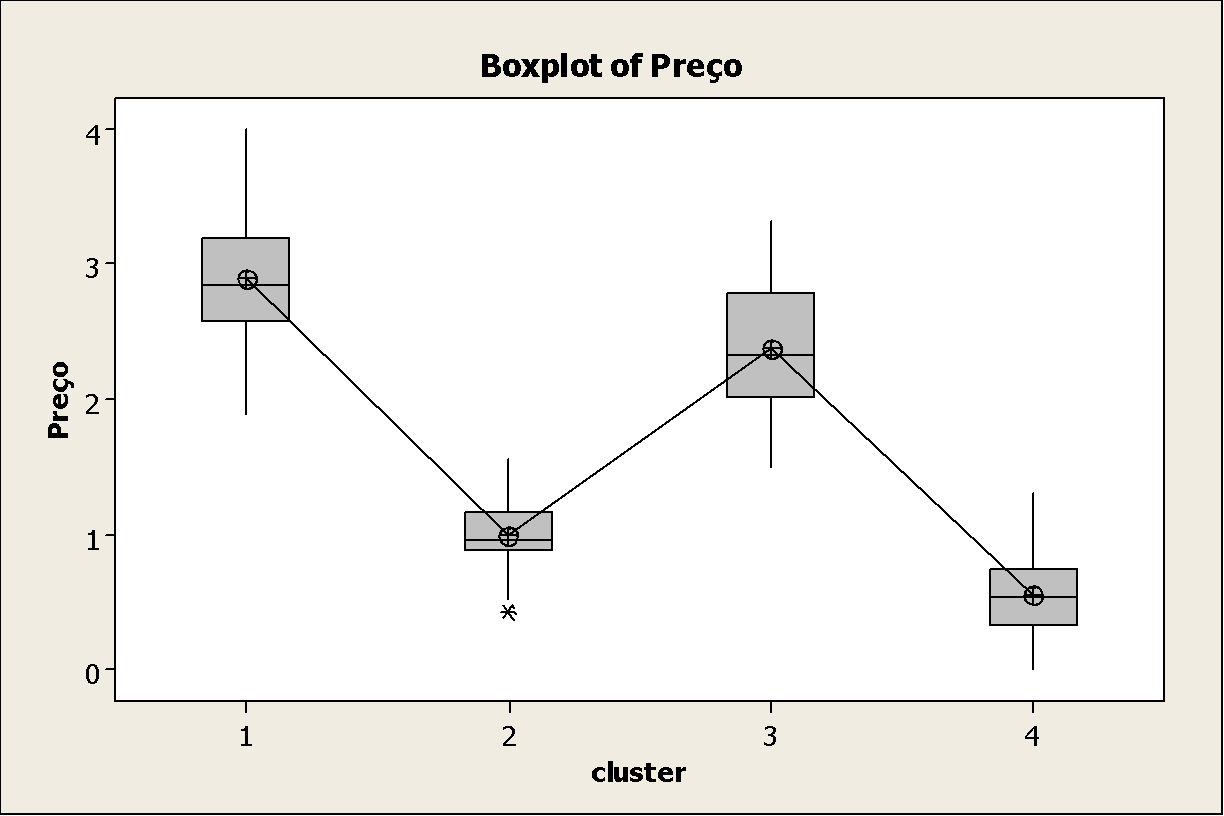
\includegraphics[width=0.45\textwidth]{Imagens/preco_vs_cluster}
\par\end{centering}

}\subfloat[\label{fig:cluster-vs-utilitario}Cluster vs Utilitário: Teste One-way
ANOVA indica Valor $p=0$ e $R_{adj}=86,28\%$]{\begin{centering}
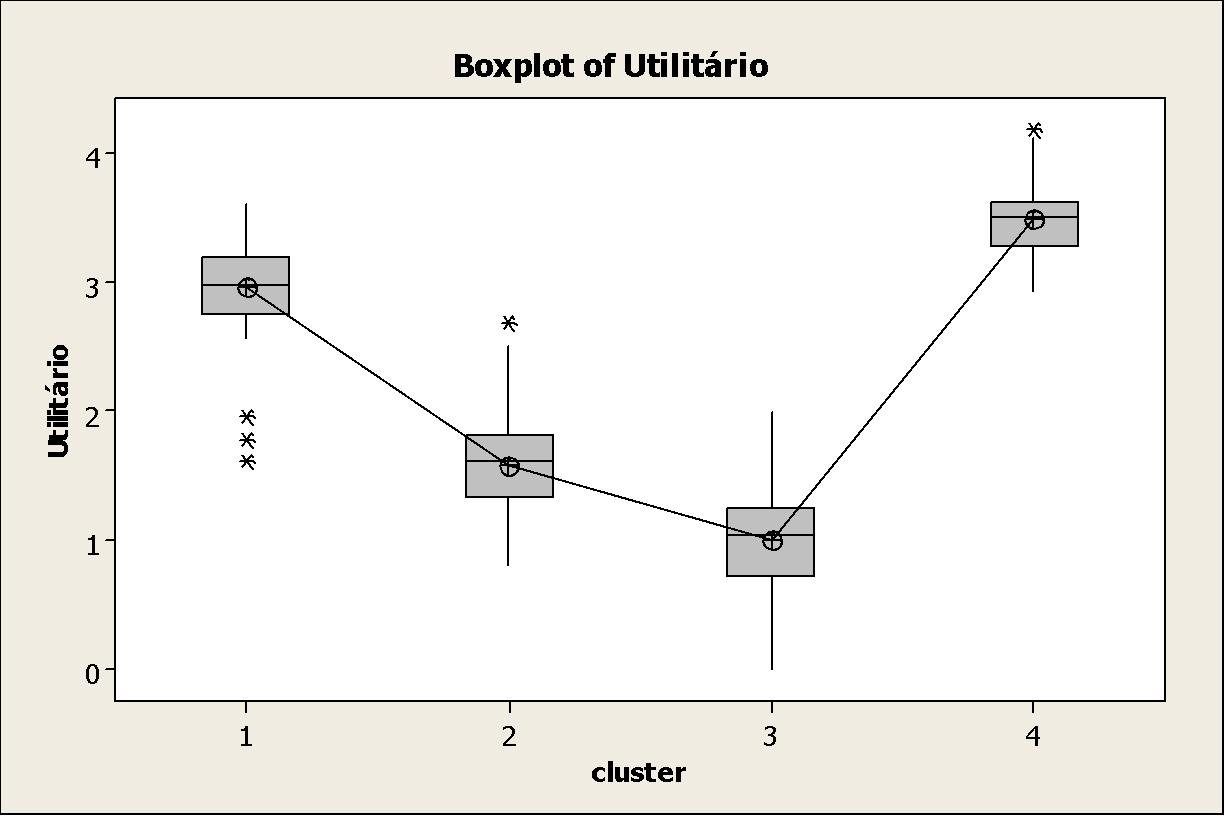
\includegraphics[width=0.45\textwidth]{Imagens/utilitario_vs_cluster}
\par\end{centering}

}
\par\end{centering}

\begin{centering}
\subfloat[\label{fig:boxplot-cluster-vs-imagem}Cluster vs Imagem: Teste One-way
ANOVA indica Valor $p=0$ e $R_{adj}=89,87\%$]{\begin{centering}
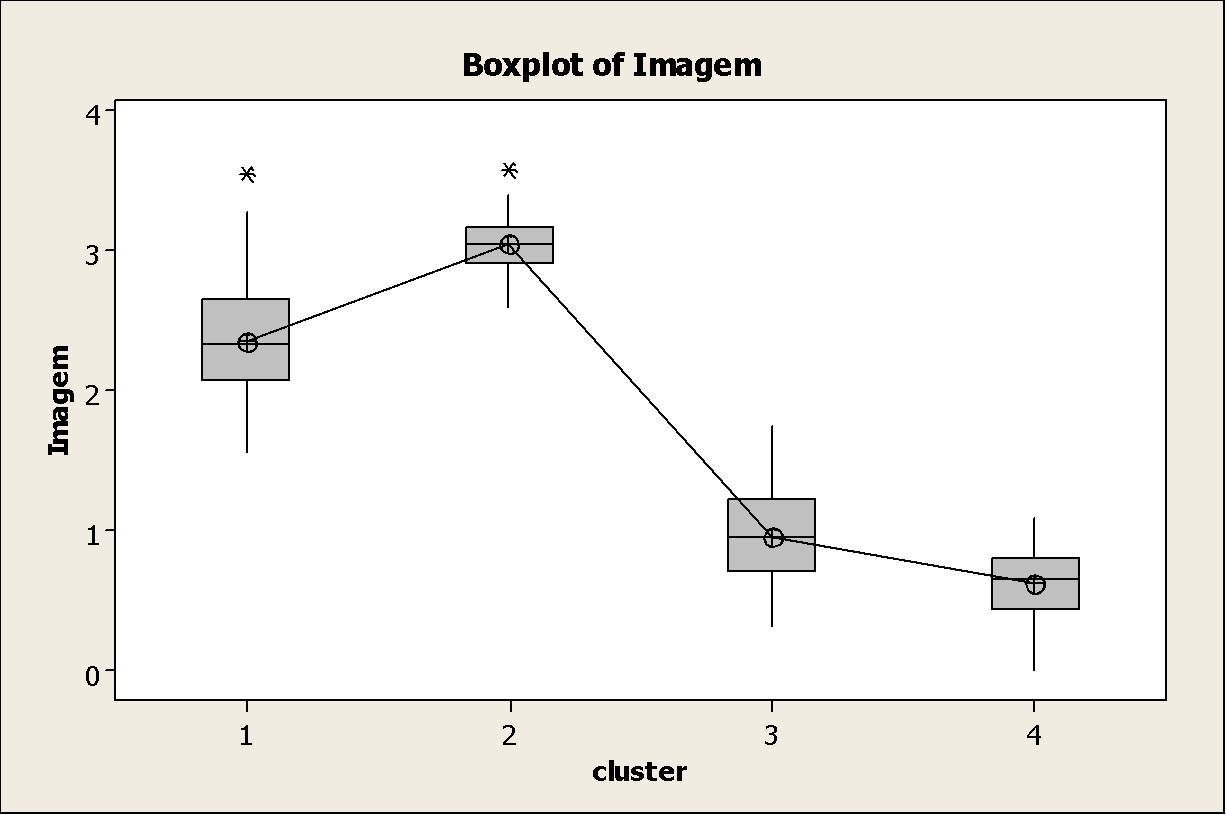
\includegraphics[width=0.45\textwidth]{Imagens/imagem_vs_cluster}
\par\end{centering}

}
\par\end{centering}

\caption{Gráficos de boxplot de variáveis vs \emph{Cluster}}
\end{figure}

\subsection{Imagem}

A imagem é um elemento de marketing mais associado ao marketing transformativo,
e sendo assim, mais voltada para o fator emocional do indivíduo. O
cluster \emph{\nomeCb{}} possui uma forte relação com essa variável,
demonstrado visualmente pelo boxplot da figura \ref{fig:boxplot-cluster-vs-imagem}
e também pelo teste one-way ANOVA do mesmo, com valor $p=0$ e a correlação
$R_{adj}=89,87\%$.

Nos clusters \emph{\nomeCc{}} e \emph{\nomeCd{}} existe uma forte
resistência a \emph{Imagem}, o que pode indicar que uma campanha publicitária
focada só nesse fator não seria bem aceita por uma parcela significativa
da população, constituídas pelos clusters mencionados, cuja soma representa
mais de 30\% de todo o espaço amostral.

Tendo isso em vista, apesar do protótipo 3 possuir forte correlação
com o grupo dos \emph{\nomeCb{}}, parece que uma propaganda baseada
nesse protótipo seria pouco abrangente nos clusters mencionados anteriormente. 

\subsection{Preço}

O teste t-Student para o preço tem valor $p=0$, indicando que há também relação
entre o preço e os clusters. Na figura \ref{fig:cluster-vs-preco},
demonstra-se que os clusters \emph{\nomeCa{}} e o \emph{\nomeCc{}}
seguem o indicador preço, enquanto o mesmo não pode ser dito nos
clusters \emph{\nomeCb{}} e \emph{\nomeCd{}}. Isso pode indicar que o preço não
é um fator decisivo na compra desses últimos, e uma estratégia publicitária
para eles não envolve o apelo popular (custo) do carro.

Já para o cluster dos \emph{\nomeCc{}}, o único apelo possível é a questão
popular, isto é, é um cluster que não se relaciona com as outras variáveis
alvos deste estudo.

\subsection{Utilitário}

O fator utilitário quando testado com relação ao cluster, indica por
meio do teste t-Student um valor $p=0$ e pelo boxplot, figura \ref{fig:cluster-vs-utilitario},
indica maior relação com o cluster \emph{\nomeCd{}} e com o cluster
\emph{\nomeCa{}}. 

Os \emph{\nomeCd{}} são o menor dos clusters em número total de amostras,
indicando que uma campanha informativa, voltada para as questões utilitárias
do veículo seria eficaz nesse grupo. Entretanto, focar nele seria
atingir uma pequena parcela do espaço amostral. Já os \emph{\nomeCa{}},
apresentam características mais heterogêneas, incluindo uma relação
estreita com Imagem, tornando uma abordagem meramente informativa
de marketing não eficaz em seu caso. 

\begin{table*}
\begin{centering}
\begin{tabular}{c|c|c|c|c|c}
\hline 
Gênero/Cluster & \nomeCa{} & \nomeCb{} & \nomeCc{} & \nomeCd{} & Todos\tabularnewline
\hline 
Feminino & 25,64 & 34,62 & 74,19 & 81,25 & 47,60\tabularnewline
\hline 
Masculino & 74,36 & 65,38 & 25,81 & 18,75 & 52,40\tabularnewline
\hline 
\emph{Total} & 100 & 100 & 100 & 100 & 100\tabularnewline
\hline 
\end{tabular}
\par\end{centering}

\caption{\label{tab:genero-vs-cluster}Tabela de Análise Chi-quadrado ($\chi^{2}=52,45$;$DF=3$)
Gênero x Cluster. Valor $p=0$.}
\end{table*}

\subsection{Gênero}

A tabela \ref{tab:genero-vs-cluster}, demonstra a dispersão de gênero
ao longo dos clusters sob a perspectiva da análise Chi-quadrado. Para
essa análise, o valor p encontrado é 0, indicando que há correlação
entre gênero e cluster. 

\begin{figure}[h]
\begin{centering}
\subfloat[\label{fig:genero-vs-utilitario}Genero vs Utilitário: Teste t-Student com
$p=0,23$.]{\begin{centering}
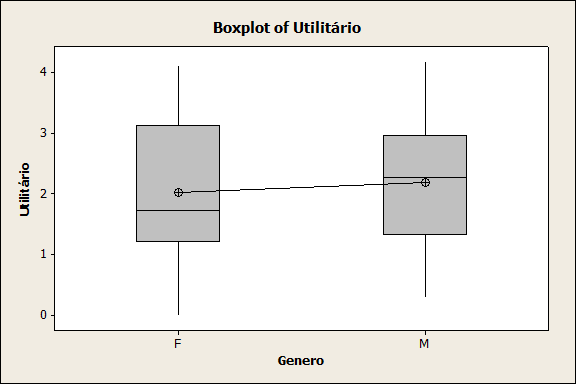
\includegraphics[width=0.45\textwidth]{Imagens/genero_vs_utilitario}
\par\end{centering}

}\subfloat[\label{fig:genero-vs-preco}Gênero vs Preço: Teste t-Student com $p=0,01$.]{\begin{centering}
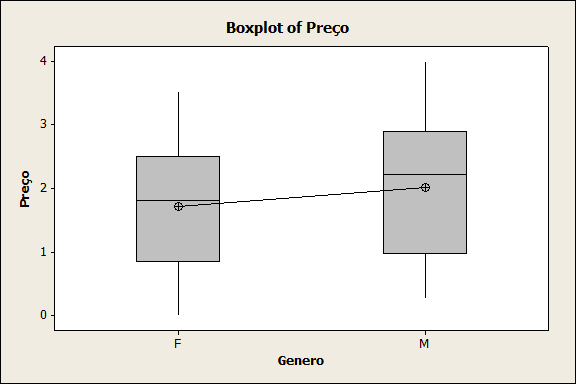
\includegraphics[width=0.45\textwidth]{Imagens/genero_vs_preco}
\par\end{centering}

}
\par\end{centering}

\begin{centering}
\subfloat[\label{fig:boxplot-genero-vs-imagem}Boxplot Gênero vs Imagem: Teste t-Student
com $p=0$.]{\begin{centering}
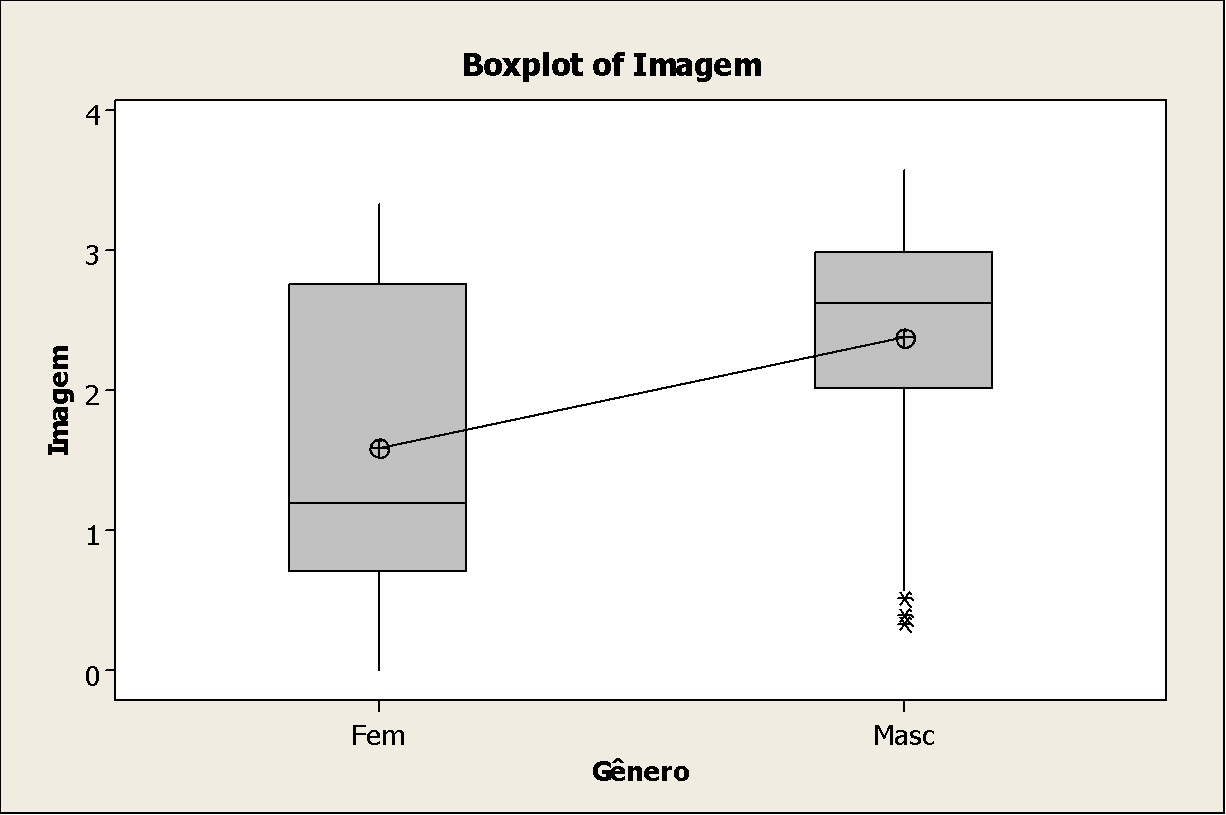
\includegraphics[width=0.45\textwidth]{Imagens/imagem_vs_genero}
\par\end{centering}

}
\par\end{centering}

\caption{Boxplots de Gênero em relação a outras variáveis.}
\end{figure}

Observa-se forte tendência ao gênero \emph{Masculino} nos clusters
\emph{\nomeCa{}} e \emph{\nomeCb{}}, caracterizados sobretudo pela existência
de relação de Imagem com o cluster, e no caso do cluster \emph{\nomeCa{}},
também pela variáveis \emph{Preço} e \emph{Utilitário}.

Quanto ao gênero \emph{Feminino}, tem-se uma maior concentração nos
clusters \emph{\nomeCc{}}, caracterizado por pessoas que não possuem preferência
específica por carros e no cluster \emph{\nomeCd{}}. Podemos assim considerar
que as mulheres da população concentram-se mais no fator \emph{Utilitário}
do protótipo? Não. A figura \ref{fig:genero-vs-utilitario} descarta
essa relação, também demonstrada pelo teste t-Student da relação,
cujo valor $p=0,23$ indica que a hipóteste nula, $H_{0}$, é aceita.


\subsubsection{Gênero e Preço}

O teste t-Student para \emph{Gênero} e \emph{Preço} obtém $p=0,01$ o que indica
correlação entre ambos. A relação em questão é, conforme vista na
figura \ref{fig:genero-vs-preco}, uma relação \emph{negativa} entre
o gênero \emph{Feminino} e a variável \emph{Preço}. Conclui-se que
as mulheres ligam menos para o aspecto \emph{Preço} do carro que os
homens para essa amostra. 

Sabe-se que uma campanha publicitária com foco em \emph{Preço} atingiria
diretamente o grupo dos \emph{\nomeCc{}} que é um dos grupos mais
homogêneos. Entretanto, o fato de haver um fator de indiferença do
gênero feminino para essa variável dificulta mais ainda o marketing
focado para um gênero. Ainda mais que na figura mencionada, vê-se
que a variável \emph{Preço} possui grande variabilidade no gênero masculino.
Conclui-se que uma publicidade informativa voltada a \emph{Preço} além
de dificultosa, seria pouco eficaz no que toca \emph{Gênero}.


\subsubsection{Gênero e Imagem}

Sabendo-se que há relação de \emph{Gênero} e \emph{Cluster}, podemos assim focar
parcialmente a estratégia de propaganda em gêneros, podendo assim
veicular em meios mais associados ao gênero em questão. 

Por exemplo, assumindo-se que o público feminino que assiste jogos
do campeonato brasileiro seja inferior ao masculino, faria sentido
veicular uma propaganda do cluster \emph{\nomeCc{}} ou do cluster
\emph{\nomeCd{}} no intervalo das partidas do mesmo? Pouco provável,
por isso o gênero pode ser fator determinante na estratégia adotada
de marketing para a campanha publicitária do protótipo.

Para tirar-se a questão a limpo, basta olhar o boxplot de imagem em
função ao gênero, da figura \ref{fig:boxplot-genero-vs-imagem}, onde
há uma forte associação ao gênero masculino nas notas mais altas de
imagem, indicando que uma estratégia de marketing para imagem, deve
provavelmente levar o gênero em consideração. Aplicando-se o teste t-Student
na amostra, obtêm-se um valor $p=0$, elucidando assim
que aceita-se $H_{a}$ na análise de ambos.

\begin{center}
\begin{table*}
\begin{centering}
\begin{tabular}{c|c|c|c|c|c}
\hline 
Filhos/Cluster & \nomeCa & \nomeCb & \nomeCc & \nomeCd & Todos\tabularnewline
\hline 
Não & 53,85 & 60,26 & 74,19 & 50 & 60,40\tabularnewline
\hline 
Tem & 46,15 & 39,74 & 25,81 & 50 & 39,60\tabularnewline
\hline 
\emph{Total} & 100 & 100 & 100 & 100 & 100\tabularnewline
\hline 
\end{tabular}
\end{centering}
\caption{\label{tab:filhos-vs-cluster}Tabela de Análise Chi-quadrado ($\chi^{2}=7,78$;$DF=3$),
Filhos x Cluster. Valor $p=0,05$.}
\end{table*}
\end{center}

\subsection{Filhos}

A tabela \ref{tab:filhos-vs-cluster}, demonstra a dispersão de gênero
ao longo dos clusters sob a perspectiva da análise Chi-quadrado. Para
essa análise, o valor $p=0,05$. Ou seja, há relação entre ter filhos
e cluster. 

Sabe-se também que o valor p para o Chi-quadrado de \emph{Estado Civil}
vs \emph{Clusters} indica é $0,96$. Isto é, a hipótese $H_{0}$ é
aceita, e não há relação entre ambos. Sendo assim, conclui-se que
independente do estado civil, há uma questão importante a ser abordada
na campanha publicitária: possui ou não filhos.

Os clusters \emph{\nomeCb{}} e \emph{\nomeCc{}} possuem uma população majoritariemente
sem filhos, enquanto os \emph{\nomeCa{}} e \emph{\nomeCd{}} são ``meio a meio''. 

A existência dessa variável pode então influenciar parcialmente uma
publicidade direcionada, principalmente para um marketing transformativo.

% WARNING - Removido por excesso de texto no trabalho!
%\begin{center}
%\begin{table*}
%\begin{centering}
%\begin{tabular}{c|c|c|c|c|c}
%\hline 
%Pequeno/Cluster & \nomeCa & \nomeCb & \nomeCc & \nomeCd & Todos\tabularnewline
%\hline 
%Não & 73,08 & 76,92 & 100 & 75 & 81,20\tabularnewline
%\hline 
%Sim & 26,92 & 23,08 & 0 & 25 & 18,80\tabularnewline
%\hline 
%\emph{Total} & 100 & 100 & 100 & 100 & 100\tabularnewline
%\hline 
%\end{tabular}
%\end{centering}

%\caption{\label{tab:tamanho-vs-cluster}Tabela de Análise Chi-quadrado ($\chi^{2}=19,47$;$DF=3$),
%Prefere Carro Pequeno vs Cluster. Valor $p=0,0$.}
%\end{table*}
%\end{center}

%\subsection{Prefere Carro Pequeno}


%O tamanho do carro é um fator importante de marketing? Sim, porque
%na tabela \ref{tab:tamanho-vs-cluster} há uma intensa relação entre
%as variáveis \emph{Carro Pequeno} e \emph{Cluster}.

%Para os \emph{\nomeCc{}} e \emph{\nomeCd{}} há predominância daqueles que não
%gostariam de um carro pequeno, enquanto nos clusters \emph{\nomeCa{}} e
%\emph{\nomeCb{}} é o oposto. 

%Especialmente no cluster \emph{\nomeCc{}} a relação é tão forte que não
%há preferência por carros pequenos. Então, uma campanha transformativa
%para esses grupos deve levar em consideração o espaço do carro, uma
%vez que há relação entre ambos.

